\documentclass[a4,11pt]{article}
\usepackage{geometry}
\geometry{a4paper, top=10mm, left=20mm, right=20mm, bottom=10mm}
\pagenumbering{gobble}
\setlength\parindent{0pt}
\usepackage[german]{babel}
\usepackage[utf8]{inputenc}


\usepackage{multicol} % Spalten
\usepackage{color} % Farben
\usepackage[hyphens]{url} % Internetadresse (mit automatischer Trennung)
\usepackage{enumitem} % Aufzählungen




% Mathesymbole
\usepackage{amsmath, amsthm, amssymb}
\usepackage{bm} % fette Schrift in Matheumgebung
\usepackage{siunitx}

% Bilder
\usepackage{caption}
\usepackage{graphicx, wrapfig}
\usepackage{subcaption} % Bilder in Gruppe einzeln benennen

\DeclareMathOperator\erf{erf}

\usepackage[
labelfont=bf,        % Tabelle x: Abbildung y: ist jetzt fett
font=small,          % Schrift etwas kleiner als Dokument
width=0.9\textwidth, % maximale Breite einer Caption schmaler
]{caption}
	\title{What's Happening?}
\begin{document}
%	\maketitle
\begin{figure}[h]
	\centering
	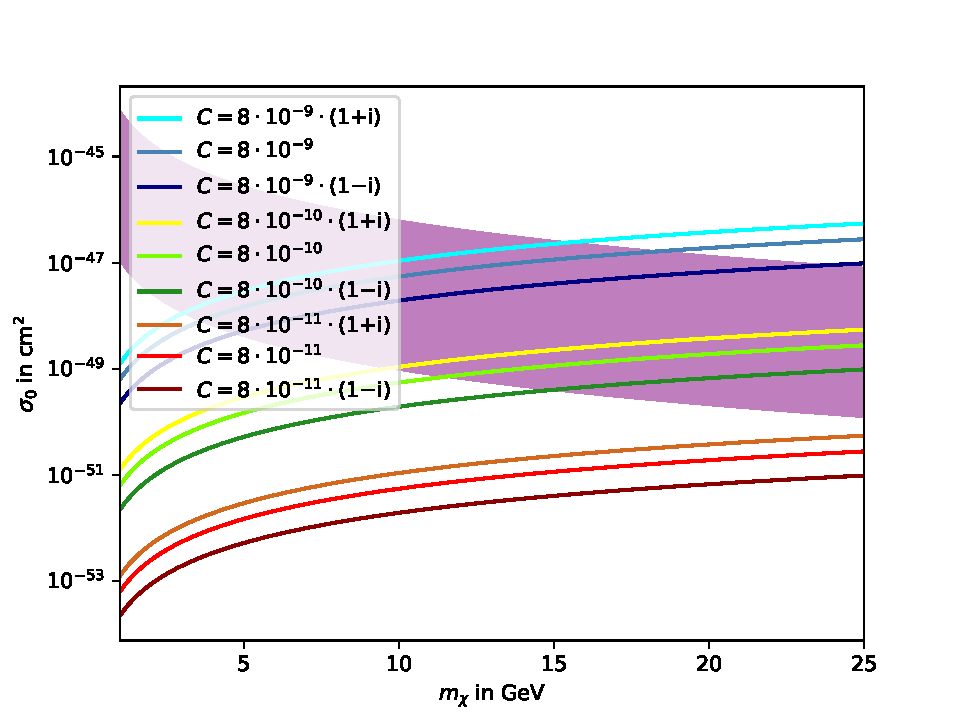
\includegraphics[width=.75\textwidth]{SigmaNull1.pdf}
	\caption{$q_\chi = q_l = 1$, $m_{Z'} = 2m_\chi$, $2\cdot10^{-3}\leq g'\leq10^{-2}$}
\end{figure}
\begin{figure}[h]
	\centering
	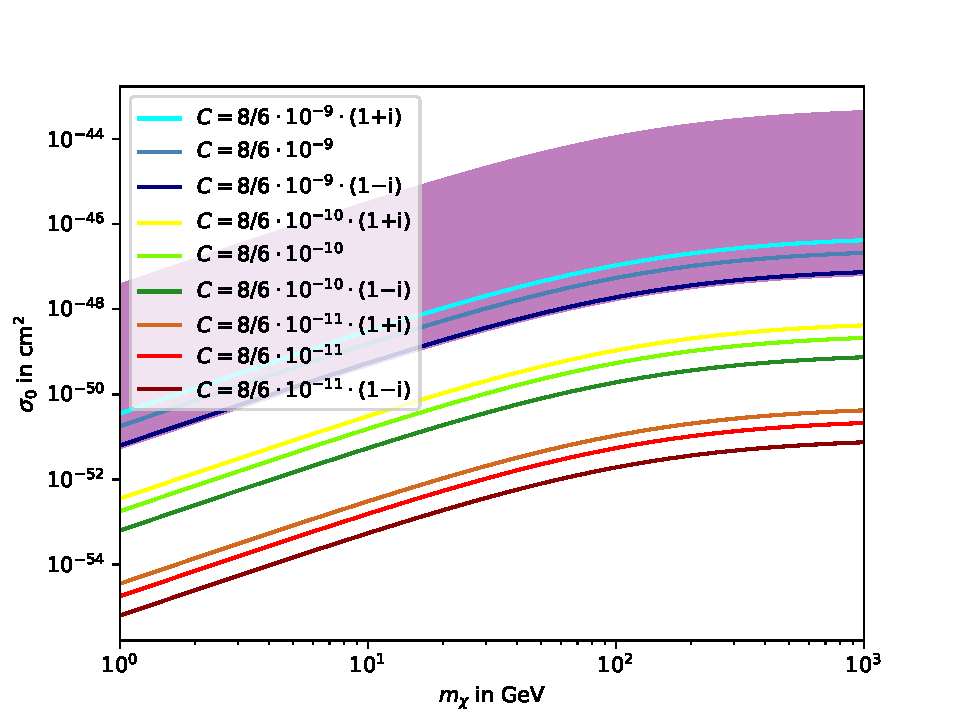
\includegraphics[width=.75\textwidth]{SigmaNull2.pdf}
	\caption{$q_\chi = \frac{1}{6}$, $q_l = 1$, $m_{Z'} = 2m_\chi$, $\SI{540}{\giga\electronvolt}\leq\frac{m_{Z'}}{g'}\leq\SI{4.9}{\tera\electronvolt}$}
\end{figure}
\begin{align*}
	\mathcal{L} = C(\bar{\chi}\gamma_\mu\chi)(\bar{s}_L\gamma^\mu b_L) + C^*(\bar{\chi}\gamma_\mu\chi)(\bar{b}_L\gamma^\mu s_L)
\end{align*}
\begin{align*}
	\sigma_{0,Z'} &= \frac{\mu_{\chi A}^2}{\pi A^2}|Z\cdot C_p + (A-Z)\cdot C_n|^2 \\
	&= \frac{\mu_{\chi A}^2}{\pi A^2}(2A-Z)^2\cdot\left(\text{Re}(V_{cd}^*V_{td}C)\right)^2 \\
	\sigma_{0,\text{Loop}} &= \frac{\mu_{\chi A}^2}{\pi A^2}\left(\frac{Z\alpha_{em}}{3\pi}\frac{q_\chi q_l{g'}^2}{m_{Z'}^2}\log\left(\frac{m_\mu^2}{m_\tau^2}\right)\right)^2
\end{align*}
\clearpage
\begin{figure}[h]
	\centering
	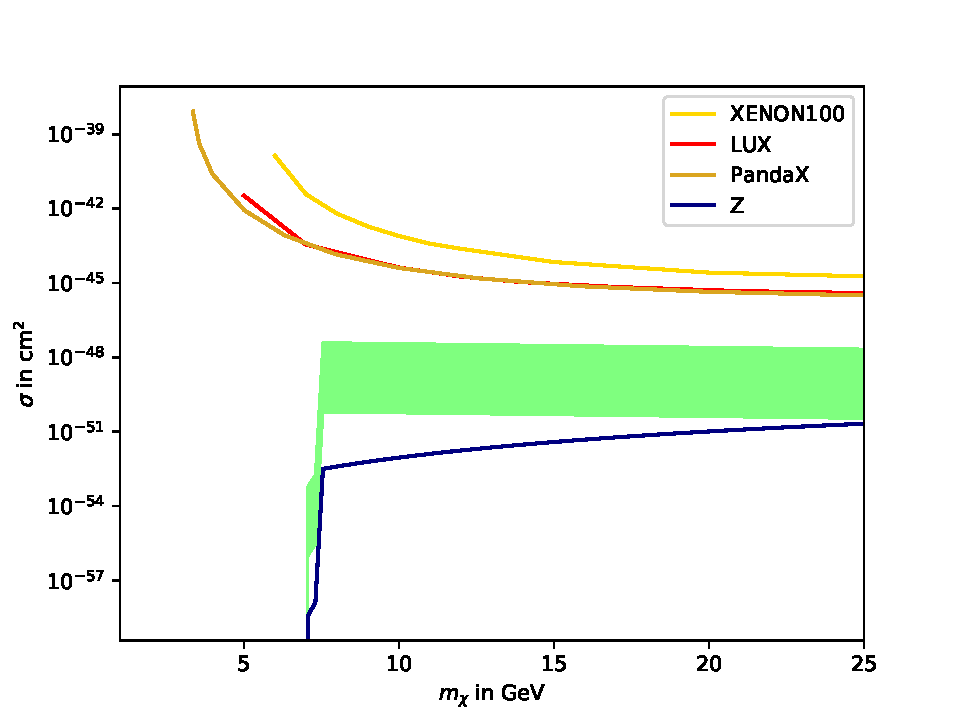
\includegraphics[width=.75\textwidth]{CrossSection.pdf}
	\caption{$q_\chi = q_l = 1$, $m_{Z'} = 2m_\chi$, $2\cdot10^{-3}\leq g'\leq10^{-2}$, $E_{min} = \SI{0}{\kilo\electronvolt}, E_{max} = \SI{10}{\kilo\electronvolt}$}
\end{figure}
\begin{align*}
	\frac{d\sigma}{dE_R} &= \frac{m_A}{2\pi v^2}|M|^2F(E_R) = \frac{m_A}{2v^2}\frac{A^2}{\mu_{\chi A}^2}\sigma_0 F(E_R) \\
	\langle\frac{d\sigma}{dE_R}\rangle &= \frac{m_A}{2}\frac{A^2}{\mu_{\chi A}^2}\sigma_0 F(E_R)\int_{v_{min}}^{\infty}dv\ \frac{f(v)}{v} \\
	&= \frac{m_A}{2}\frac{A^2}{\mu_{\chi A}^2}\sigma_0 \frac{F(E_R)}{2v_E}\left[\erf{\left(\frac{v_E-v_{min}}{v_0}\right)}+\erf{\left(\frac{v_E+v_{min}}{v_0}\right)}\right] \\
	\langle\sigma\rangle &= \frac{m_A}{2}\frac{A^2}{\mu_{\chi A}^2}\sigma_0 \frac{1}{2v_E}\int_{E_{min}}^{E_{max}}dE_R\ F(E_R)\left[\erf{\left(\frac{v_E-v_{min}(E_R)}{v_0}\right)}+\erf{\left(\frac{v_E+v_{min}(E_R)}{v_0}\right)}\right]
\end{align*}
\end{document}